% -  -  -  -  -  -  -  -  -  -  -  -  -  -  -  -  -  -  -  -  -  -  -  -  -  -  -  -  -  -  -  -  -  -  -  -  -  -  -  -  -  -  -  -  -  -  -  -  -  -  -  -  - %
%-----Chapter 3: Kalman Filtering-------%
\chapter{Kalman Filtering}

\section{Linear Kalman Filter}
There exists a recursive Kalman filter algorithm for discrete time systems.\cite{IntroKF} This ongoing Kalman filter cycle can be divided into two groups of equations
\newline
\begin{enumerate}
	\item Time update equations
	\begin{equation}\label{TupEq}
		\begin{aligned}
    			\hat{x}_{k}^{-} &= A\hat{x}_{k-1}+Bu_{k-1} \\
    			P_{k}^{-} &= AP_{k-1}A^{T}+Q
  		\end{aligned}
	\end{equation}
	\item Measurement update equations
	\begin{equation}\label{MupEq}
		\begin{aligned}
    			K_{k} &= P_{k}^{-}H^{T}(HP_{k}^{-}H^{T}+R)^{-1} \\
    			\hat{x}_{k} &= \hat{x}_{k-1}^{-}+K_{k}(z_{k}-H\hat{x}_{k}^{-}) \\
			P_{k} &= (I-K_{k}H)P_{k}^{-}
  		\end{aligned}
	\end{equation}
\end{enumerate}

To test this algorithm and to learn something about applying the Kalman filter on linear systems we created an example. A detailed description of the following example can be found in appendix \ref{ExampleKF}. \newline 
We consider a linear, timeinvariant model, given by the following circuit diagram in figure \ref{KFcircuit}.
\begin{figure}[htbp]
	\centering
	\begin{pspicture}(-3,-1)(9,5)
		%nodes
			\pnode(-2,4){A}		\pnode(-2,0){B}		\pnode(8,4){C0}		\pnode(8,0){D}
			\pnode(3,4){A2}		\pnode(3,2){M}		\pnode(3,0){B2}	\pnode(6,4){C2}
			\pnode(6,0){D2}
		%elements
			\coil[intensitylabel=$i_L$,labeloffset=-0.2](A)(A2){$L$}
			\capacitor[tensionlabel=$U_1$,tensionlabeloffset=-1.2,tensionoffset=-0.8,%
					intensitylabel=$i_1$,dipoleconvention=generator](A2)(M){$C_1$}
			\resistor[tensionlabel=$U_R$,tensionoffset=0.8,labeloffset=-0.5](B2)(M){$R$}
			\capacitor[tensionlabel=$U_2$,tensionlabeloffset=-1.2,tensionoffset=-0.8,%
					intensitylabel=$i_2$,dipoleconvention=generator](C2)(D2){$C_2$}
		%wires
			\wire(B)(D)		\wire(A2)(C0)
			\pscircle[fillstyle=solid](A){0.075}
			\pscircle[fillstyle=solid](B){0.075}
			\pscircle[fillstyle=solid](C0){0.075}
			\pscircle[fillstyle=solid](D){0.075}
		%tension
			\tension(A)(B){$U_{in}$}
			\tension(C0)(D){$U_{out}$}
	\end{pspicture}
    	%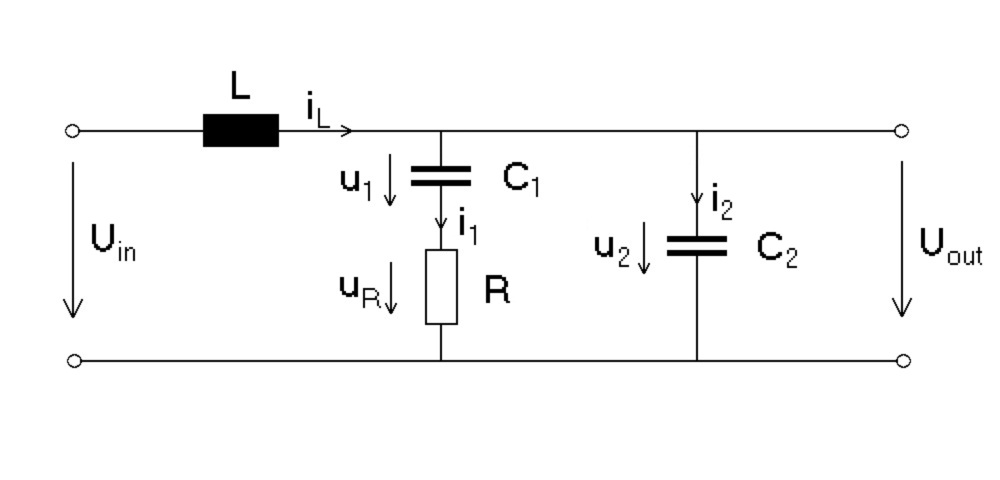
\includegraphics[width=12cm]{./3_KalmanFilter/circuit_diagram.jpg}
  	\caption{Example: Linear electrical circuit.}
  	\label{KFcircuit}
\end{figure}
First we added process noise and measurement noise to the system output. The aim is to get an estimation of the noisy output. Therefore we applied the Kalman filter algorithm based on the equations \ref{TupEq}. In the figure \ref{KFchart}, above we can see the input signal and the ideal measurement of the output signal. That ideal measurement includes process noise, which can obviously not be filtered by the Kalman filtering algorithm. Below one can see the noisy measurement on the left side and the filtered output on the right side.
\begin{figure}[htbp]
	\centering
    	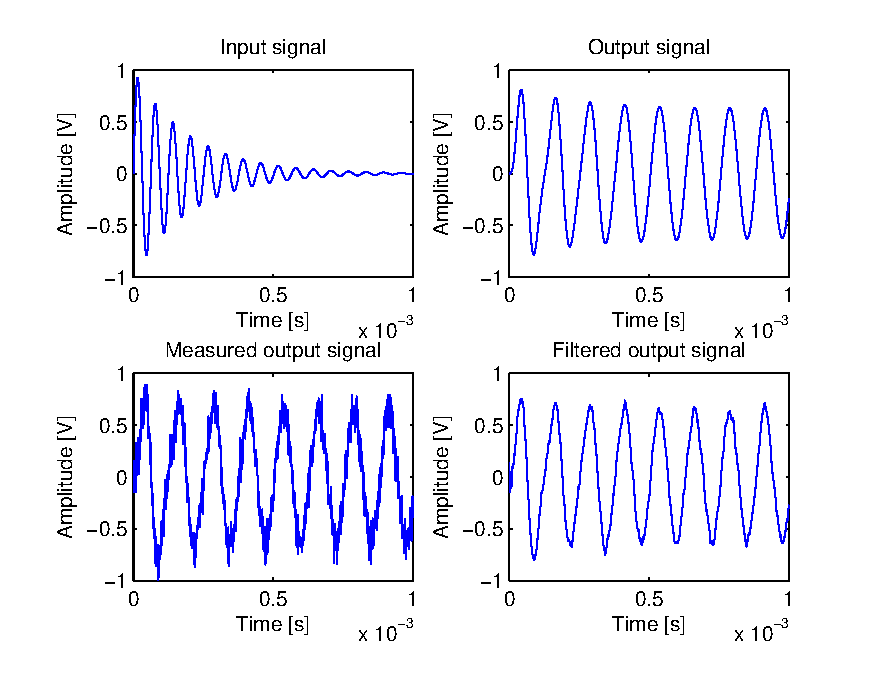
\includegraphics[width=12cm]{./3_KalmanFilter/KFchart}
  	\caption{Example: Input signal, output signal, noisy output, and filtered output.}
  	\label{KFchart}
\end{figure}

\section{Extended Kalman Filter (EKF)}

In the section above we discussed the usage of a Kalman filter on linear systems. Most systems, including the motion equations of our robots, however are nonlinear. Nevertheless linearizing our system around the current estimate still makes our Kalman filter useful and leads to the concept of the extended Kalman filter \cite{IntroKF}. The recursive equations are quite similar to those of the linear Kalman filter
\newline
\begin{enumerate}
	\item Time update equations
	\begin{equation}\label{TupEqEKF}
		\begin{aligned}
    			\hat{x}_{k}^- &= f(\hat{x}_{k-1},u_{k-1},0) \\
    			P_{k}^{-} &= A_kP_{k-1}A_k^T+W_k Q_{k-1} W_k^T
  		\end{aligned}
	\end{equation}
	\item Measurement update equations
	\begin{equation}\label{MupEqEKF}
		\begin{aligned}
    			K_{k} &= P_{k}^- H_k^T(H_k P_k^- H_k^T+V_k R_k V_k^T)^{-1} \\
    			\hat{x}_k &= \hat{x}_{k-1}^- + K_{k}(z_k - h(\hat{x}_k^-, 0)) \\
			P_k &= (I-K_k H_k)P_k^-
  		\end{aligned}
	\end{equation}
\end{enumerate}

The function \(f(\hat{x}_k,u_k,w_k)\) contains the system's nonlinear dynamics where \(w_k\) represents the current process noise and \(h(\hat{x}_k, v_k)\) denotes the nonlinear state-to-output relationship with the measurement noise \(v_k\). Furthermore the matrices \(A_k\), \(H_k\), \(W_k\) and \(V_k\) are linearizations, i.e. partial drivatives, of their respective functions at time step \(k\)
\newline
\begin{enumerate}
	\begin{equation}\label{Linearizations}
		\begin{aligned}
    			A_{i,j}&= \frac{\partial f_i}{\partial x_j}(\hat{x}_{k-1},u_{k-1},0) \\
    			H_{i,j}&= \frac{\partial h_i}{\partial x_j}(\hat{x}_{k-1},u_{k-1},0) \\
			W_{i,j}&= \frac{\partial f_i}{\partial w_j}(\tilde{x}_k,0) \\
			V_{i,j}&= \frac{\partial h_i}{\partial v_j}(\tilde{x}_k,0)
  		\end{aligned}
	\end{equation}
\end{enumerate}

We dropped the fact that all matrices should have a subscript \(k\) and that they are allowed be different at each time step. Again, before applying the theory to our simulation, we created a generic example of a nonlinear system. Further details can be looked up in section \ref{ExampleEKF}. We did essentially the same as we did for the linear system: We simulated the ideal system, then added process and measurement noise and in the last step checked whether we could get rid of our artifically added measurement noise. The results for a sample run on MATLAB are shown in figure \ref{EKFchart} below

\begin{figure}[htbp]
	\centering
    	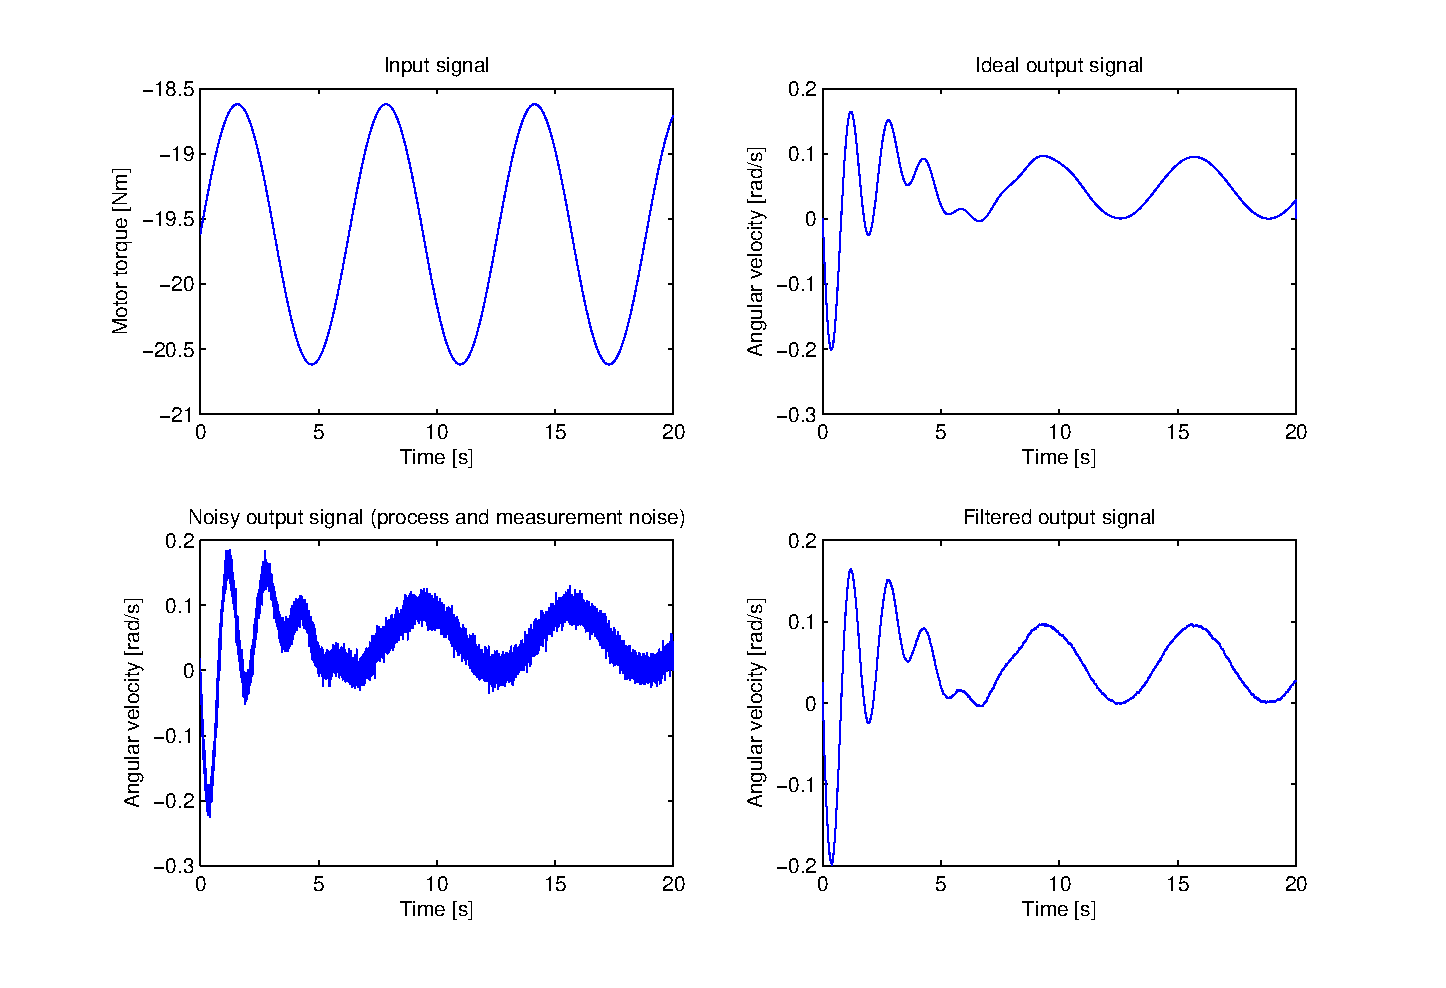
\includegraphics[width=12cm]{./3_KalmanFilter/EKFchart}
  	\caption{Example: Input signal, output signal, noisy output, and filtered output.}
  	\label{EKFchart}
\end{figure}

The two pictures above show the sinusoidal input on the left and the ideal output, i.e. without process and measurement noise, on the right. Thereunder we can see the plots of the noisy signal and the signal after it has been filtered by the extended Kalman filter. We can conclude that the extended Kalman filter too provides an acceptable performance if our measurement noise is not too big.


